\subsection{Geometria}
\label{sec:teogeom}

\begin{figure}
	\center
	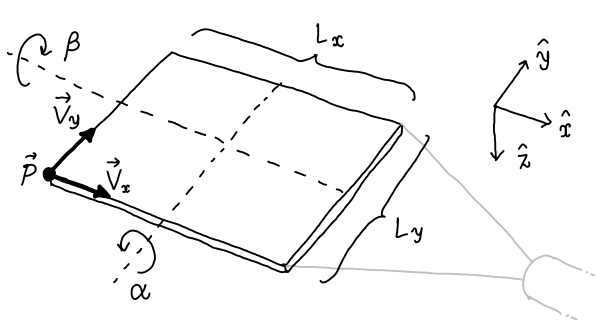
\includegraphics[width=25em]{geometriadef}
	\caption{\label{fig:geometriadef}
	Definizione del modello geometrico.
	Gli angoli $\alpha$ e $\beta$ sono nulli
	quando il lato della lastra ortogonale al loro asse di rotazione è orizzontale.
	Gli assi di rotazione sono riferiti alla lastra.}
\end{figure}

Esponiamo la modellizzazione geometrica dell'apparato ai fini di calcoli e simulazioni
(vedi \autoref{fig:geometriadef}).
Consideriamo ogni lastra di scintillatore come un parallelepipedo.
Teniamo conto dei \emph{disallineamenti} cioè della posizione arbitraria nello spazio delle lastre,
supponendo però che sia poco diversa da quella ideale di lastre orizzontali, rettangolari e allineate verticalmente.
Chiamiamo $x$ la direzione orizzontale parallela ai tubi fotomoltiplicatori,
$y$ quella ortogonale,
$z$ la direzione verticale.
Assumiamo che la direzione verticale data dalla gravità
coincida con la media dei versori normali alle lastre.